% Readaptado de Semana 09 Clase 01 (2025-A): bases y representacion unica.
\documentclass[compacto,10pt]{pubciencias-notas}
\usepackage{comandosEPN}
\usepackage{tikz}
\usetikzlibrary{babel}
\autor{Departamento de Formación Básica}
\materia{Álgebra Lineal}
\nota{Semana 10 Clase 01}
\fecha{Semestre 2026-B}
\logouno[1.1cm]{Logo_EPN.eps}
\logodos[1.7cm]{Logo_DFB.eps}
\definecolor{colordef}{cmyk}{0.81,0.62,0.00,0.22}
\raggedbottom

\begin{document}
\encabezado
\vspace*{-8mm}
\setcounter{section}{3}
\section{Espacios vectoriales}
\subsection{Bases de espacios vectoriales}

Los conceptos de generación e independencia lineal permiten caracterizar
conjuntos que representan de manera única los vectores de un espacio.
Un conjunto generador puede contener vectores redundantes, mientras que
un conjunto linealmente independiente puede generar un subespacio propio.
La noción de base exige ambas propiedades simultáneamente.
En lo que sigue, se consideran operaciones usuales y escalares reales.

\begin{defi}[Espacio vectorial de dimensión finita]
    Un espacio vectorial real $V$ es de \textbf{dimensión finita} si
    existe un conjunto finito $S\subseteq V$ tal que $\spn(S)=V$;
    es decir, si $V$ admite un conjunto generador con un número finito
    de elementos.
\end{defi}

En estas dos clases se supondrá que $V$ es de dimensión finita.
Se empleará la abreviatura \textbf{l.i.} para ``linealmente independiente''.

\begin{defi}[Base]\label{sem10cl01:base}
    Sea $V$ un espacio vectorial real. Un conjunto finito
    $B=\{v_1,\ldots,v_k\}\subseteq V$ es una \textbf{base de $V$} si:
    \begin{enumerate}
        \item $B$ genera $V$, es decir, $\spn(B)=V$;
        \item $B$ es linealmente independiente (l.i.).
    \end{enumerate}
\end{defi}

La primera condición garantiza la existencia de una representación de cada
vector de $V$ como combinación lineal de los elementos de $B$; la segunda
excluye la presencia de vectores redundantes. Toda afirmación de que un
conjunto es una base debe precisar el espacio vectorial correspondiente.

\begin{ejem}[Una base no canónica de $\R^2$]\label{sem10cl01:planoR2}
    Sean $u=(1,1)$ y $v=(1,-1)$. Pruebe que $B=\{u,v\}$ es una base
    de $\R^2$.

    \textbf{Solución.} Para un vector arbitrario $(x,y)\in\R^2$, buscamos
    $\alpha,\beta\in\R$ tales que
    \[
        \alpha(1,1)+\beta(1,-1)=(x,y).
    \]
    Igualando componentes obtenemos
    \[
        \left\{\begin{aligned}\alpha+\beta&=x,\\\alpha-\beta&=y.\end{aligned}\right.
        \quad\Longrightarrow\quad
        \alpha=\frac{x+y}{2},\quad\beta=\frac{x-y}{2}.
    \]
    El sistema es compatible para todo $(x,y)\in\R^2$, por lo que $\spn(B)=\R^2$.
    Para la combinación nula $\alpha u+\beta v=(0,0)$, se toma
    $x=y=0$ y las únicas soluciones son
    $\alpha=\beta=0$; así, $B$ es linealmente independiente y, por tanto,
    es una base.

    En particular, $(3,1)=2u+v$. Geométricamente, todo desplazamiento del
    plano se expresa como suma de múltiplos de las direcciones determinadas
    por $u$ y $v$. Los coeficientes pueden ser positivos, negativos o cero.
\end{ejem}

\begin{center}
    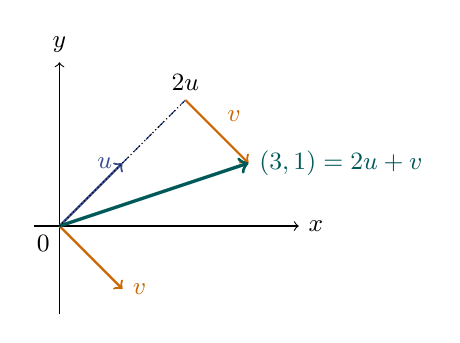
\begin{tikzpicture}[scale=0.8,every node/.style={font=\small}]
        \draw[->] (-0.4,0)--(3.8,0) node[right] {$x$};
        \draw[->] (0,-1.4)--(0,2.6) node[above] {$y$};
        \draw[->,thick,colordef] (0,0)--(1,1) node[left] {$u$};
        \draw[->,thick,orange!80!black] (0,0)--(1,-1) node[right] {$v$};
        \draw[dashed,colordef] (1,1)--(2,2);
        \draw[->,thick,orange!80!black] (2,2)--(3,1)
            node[midway,above right] {$v$};
        \draw[->,very thick,teal!70!black] (0,0)--(3,1)
            node[right] {$(3,1)=2u+v$};
        \draw[densely dotted] (0,0)--(2,2) node[above] {$2u$};
        \node[below left] at (0,0) {$0$};
    \end{tikzpicture}
\end{center}

\subsection{Una base de un subespacio}

\begin{ejem}[Una base de un plano que pasa por el origen]\label{sem10cl01:planoR3}
    Sea $P=\{(x,y,z)\in\R^3:x+y-z=0\}$. Determine una base de $P$.

    \textbf{Solución.} Como $z=x+y$, un vector genérico del plano se
    escribe
    \[
        (x,y,z)=(x,y,x+y)=x(1,0,1)+y(0,1,1).
    \]
    Así, $a=(1,0,1)$ y $b=(0,1,1)$ generan $P$. Además,
    \[
        \alpha a+\beta b=(\alpha,\beta,\alpha+\beta)=(0,0,0)
    \]
    implica $\alpha=\beta=0$. Por tanto, $B=\{a,b\}$ es una base de $P$.
    No es una base de $\R^3$: por ejemplo, $(0,0,1)$ no pertenece al plano
    y no es una combinación lineal de $a,b$.
\end{ejem}

\begin{ejem}[Matrices sujetas a una restricción]\label{sem10cl01:matrices}
    Determine una base del subespacio
    \[
        W=\left\{\begin{pmatrix}a&b\\b&c\end{pmatrix}
            \in\Mat[\R]{2}{2}:b=3a\right\}.
    \]

    \textbf{Solución.} Al sustituir la restricción $b=3a$, todo elemento
    de $W$ admite la expresión
    \[
        \begin{pmatrix}a&3a\\3a&c\end{pmatrix}
        =a\begin{pmatrix}1&3\\3&0\end{pmatrix}
        +c\begin{pmatrix}0&0\\0&1\end{pmatrix},\qquad a,c\in\R.
    \]
    Sean $M_1,M_2$ las matrices que multiplican a los parámetros $a,c$,
    respectivamente. Ambas pertenecen a $W$ y generan dicho subespacio.
    Para verificar independencia lineal, se considera la igualdad
    \[
        \alpha M_1+\beta M_2=
        \begin{pmatrix}\alpha&3\alpha\\3\alpha&\beta\end{pmatrix}
        =\begin{pmatrix}0&0\\0&0\end{pmatrix}.
    \]
    Comparando las entradas $(1,1)$ y $(2,2)$, obtenemos
    $\alpha=\beta=0$. Así, $\{M_1,M_2\}$ es una base de $W$.
    En este caso, el vector cero es la matriz nula de tamaño $2\times2$.
\end{ejem}

\begin{ejem}[Una base de polinomios]\label{sem10cl01:polinomios}
    Pruebe que $B=\{1+t,1-t\}$ es una base de $\Pol_1$.

    \textbf{Solución.} Tomemos un polinomio arbitrario $p(t)=a_0+a_1t$.
    Buscamos $\alpha,\beta\in\R$ tales que
    \[
        \alpha(1+t)+\beta(1-t)
        =(\alpha+\beta)+(\alpha-\beta)t=a_0+a_1t.
    \]
    Igualar los coeficientes de cada potencia da
    \[
        \left\{\begin{aligned}\alpha+\beta&=a_0,\\\alpha-\beta&=a_1.\end{aligned}\right.
    \]
    Para cada elección de $a_0,a_1\in\R$, el sistema tiene solución única:
    $\alpha=(a_0+a_1)/2$, $\beta=(a_0-a_1)/2$. En particular, para
    la combinación nula $\alpha(1+t)+\beta(1-t)=0_{\Pol_1}$,
    se tiene $a_0=a_1=0$, lo que implica $\alpha=\beta=0$.
    Así, $B$ genera $\Pol_1$ y es linealmente independiente; por tanto,
    es una base.
\end{ejem}

\subsection{Bases canónicas y representación única}

\begin{teo}[Bases canónicas]
    Los siguientes conjuntos son bases de los espacios indicados:
    \begin{itemize}
        \item En $\R^n$, $\{e_1,\ldots,e_n\}$, donde $e_i$ tiene
              una componente 1 en la posición $i$ y ceros en las demás.
        \item En $\Mat[\R]{m}{n}$, $\{E_{ij}:1\le i\le m,\ 1\le j\le n\}$,
              donde $E_{ij}$ tiene una entrada 1 en la posición $(i,j)$
              y ceros en las demás.
        \item En $\Pol_n$, $\{1,t,\ldots,t^n\}$.
    \end{itemize}
\end{teo}

En cada caso, las componentes, entradas o coeficientes permiten escribir
cualquier elemento como combinación de esos vectores. Al igualar esa
combinación al vector cero del espacio correspondiente, todos sus
coeficientes deben ser cero.
Por ejemplo, en $\Mat[\R]{2}{2}$,
\[
    \begin{pmatrix}a&b\\c&d\end{pmatrix}
    =aE_{11}+bE_{12}+cE_{21}+dE_{22}.
\]

\begin{teo}[Caracterización por representación única]
    Un conjunto $B=\{v_1,\ldots,v_k\}\subseteq V$ es una base de $V$
    si y solo si cada $v\in V$ se escribe de manera única como
    \[
        v=\alpha_1v_1+\cdots+\alpha_kv_k.
    \]
\end{teo}

\begin{advertencia}
    Un espacio vectorial puede admitir distintas bases. La unicidad de
    la representación de cada vector se establece \textbf{respecto de una
    base fija}.
    Por ejemplo, $\{1,t\}$ y $\{1+t,1-t\}$ son bases distintas de $\Pol_1$.
\end{advertencia}

\section{Ejercicios}

\begin{ejer}[Una base en el espacio]
    Sea $B=\{(1,1,0),(1,0,1),(0,1,1)\}\subseteq\R^3$.
    \begin{enumerate}
        \item Plantee el sistema para un vector genérico $(x,y,z)$ y
              pruebe que $B$ genera $\R^3$ y es linealmente independiente.
        \item Escriba $(2,1,3)$ como combinación de los vectores de $B$.
    \end{enumerate}
\end{ejer}

\begin{ejer}[Encontrar una base de un subespacio]
    Sea $W=\{(x,y,z)\in\R^3:x-2y+z=0\}$.
    \begin{enumerate}
        \item Exprese su vector genérico con parámetros y obtenga una
              base de $W$, verificando generación e independencia.
        \item Explique por qué esa base no es una base de $\R^3$.
    \end{enumerate}
\end{ejer}

\begin{ejer}[Una base de matrices simétricas]
    Sea $W=\{A\in\Mat[\R]{2}{2}:a_{12}=a_{21}\}$.
    \begin{enumerate}
        \item Descomponga una matriz genérica de $W$ para proponer una
              base y compruebe que el conjunto propuesto es linealmente
              independiente.
        \item Escriba $\begin{pmatrix}2&-1\\-1&3\end{pmatrix}$ como
              combinación de los elementos de su base.
    \end{enumerate}
\end{ejer}

\begin{ejer}[Una base no canónica de polinomios]
    En $\Pol_2$, considere $B=\{1,t+t^2,t^2\}$.
    \begin{enumerate}
        \item Plantee la combinación para $a_0+a_1t+a_2t^2$ y pruebe
              que tiene coeficientes únicos. Concluya que $B$ es una base.
        \item Exprese $2-t+3t^2$ como combinación de los elementos de $B$.
    \end{enumerate}
\end{ejer}

\end{document}
